% !TeX spellcheck = pl_PL

\newcommand\XOR{\mathbin{\char`\^}}
\newpage
\section{IEEE-488 and SCPI standards}
Standard IEEE-488, ogłoszony w 1973 roku, określa organizację systemów ATE (\emph{Automatic Test Equipment}), przeznaczonych do akwizycji danych i sterowania urządzeń w obiektach skupionych lub rozproszonych. Te mają zastosowanie w testowaniu wyborów, pomiarach laboratoryjnych, sterowaniu procesami przemysłowymi itp.\\
Urządzenia systemu ATE wyposażone są w układ komunikacyjny (interfejs), który umożliwia wymianę danych za pomocą łącza interfejsowego. Pracą systemu zarządza kontroler, który jest nadrzędny w stosunku do pozostałych urządzeń, które pełnią rolę przyrządów wykonawczych.\\
Standard IEEE-488 znany jest również jako GPID (\emph{General Purpose Interface Bus}). Określa on dokładnie własności elektryczne i mechaniczne interfejsu, jego protokoły i funkcje, jednak nie normuje przesyłanych treści. Tym zajmuje się uzupełnienie standardu w postaci IEEE-488.2 (1973) oraz SCPI (1990).\\\\
Protokół systemu ATE można podzielić na 3 poziomy:
\begin{itemize}
	\item Poziom 1, złożony z
	\begin{itemize}
		\item Warstwa fizyczna (GPIB), określa łącze transmisyjne i sposób przesyłania jednostek
		\item Warstwa łącza danych, dostarcza reguły dostępu do łącza, sposób adresacji itp.
	\end{itemize}
	\item Poziom 2, IEEE-488.2 kontroler $<->$ IEEE-488.2 urządzenie\\
	Standard IEEE-488.2 okresla protokół wymiany komunikatów, syntaktykę komunikatów i strukturę danych.
	\item Poziom 3, rozkazy SCPI $<->$ Interpretacja rozkazów, generacja odpowiedzi\\
	SCPI normuje treść komunikatów przesyłanych pomiędzy kontrolerem a urządzeniem.
	\item Poziom 4, Aplikacja $<->$ Wykonanie funkcji urządzenia (ale to już nas raczej nie interesuje).
\end{itemize}
\textbf{Ilustracja rozwoju standardu IEEE-488} oraz \textbf{model komunikacyjny systemu ATE}\\
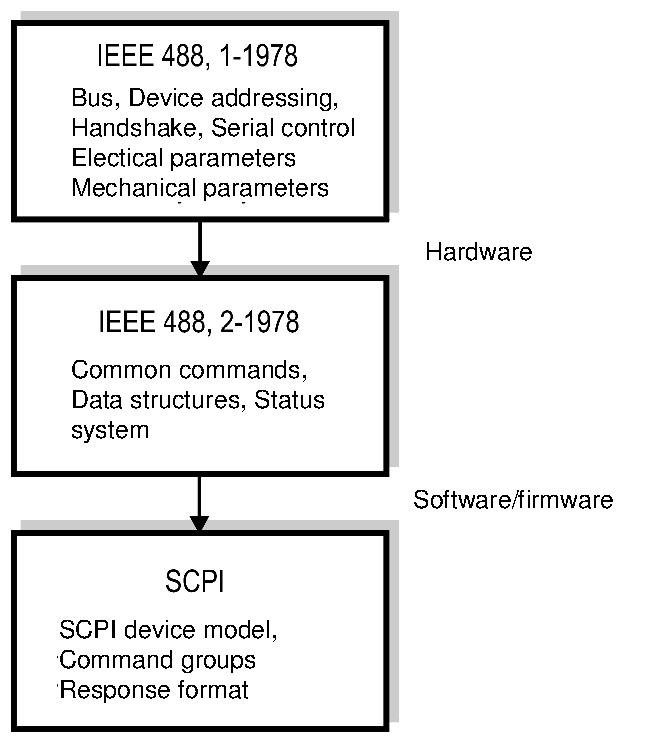
\includegraphics[width=7cm]{./wyklady/IEEE488_SCPI_17_1.pdf}
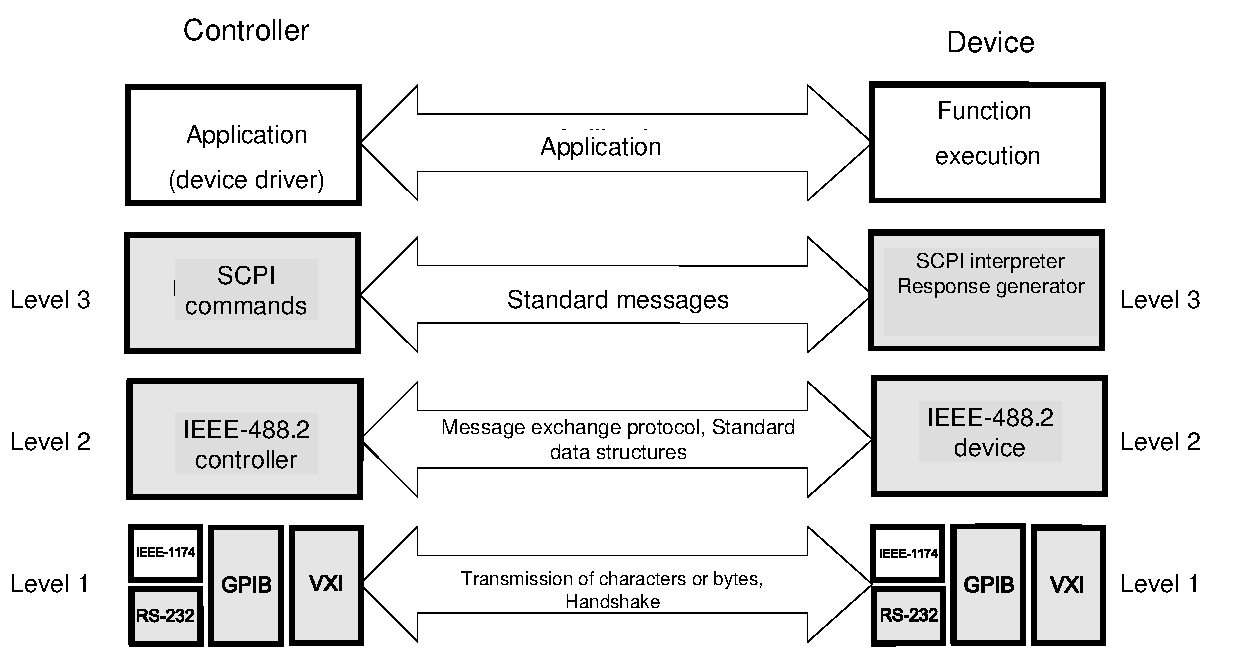
\includegraphics[width=9cm]{./wyklady/IEEE488_SCPI_18_1.pdf}

% ==============================================================
% --- Standard IEEE-488
% ==============================================================
\newpage
\subsection{IEEE-488 (GPIB)}
Standard GPIB ogłoszono w 1979 roku, jest definicją warstwy fizycznej oraz łącza danych dla systemów pomiarowo-kontrolnych, przeznaczonych do:
\begin{itemize}
	\item Testowania wyborów
	\item Pomiarów laboratoryjnych i przemysłowych
\end{itemize}

\subsubsection{Interface profile}
Standard ten określa budowę i działanie części komunikacyjnej systemu opartego na magistrali, do której można:
\begin{itemize}
	\item Podłączyć do 15 urządzeń,
	\item Rozłożonych na niewielkim obszarze (zasięg do 20 m),
	\item Maksymalna odległość między kolejnymi urządzeniami to 2 m,
	\item Wymieniających między sobą dane rzędu 300 do 500 kB / s
\end{itemize}
Komunikacją zarządza kontroler, który konfiguruje system do komunikacji, obsługuje zgłoszenia żądania obsługi i wykonuje podstawowe operacje.
\textbf{Dwie podstawowe konfiguracje systemu GPIB}\\
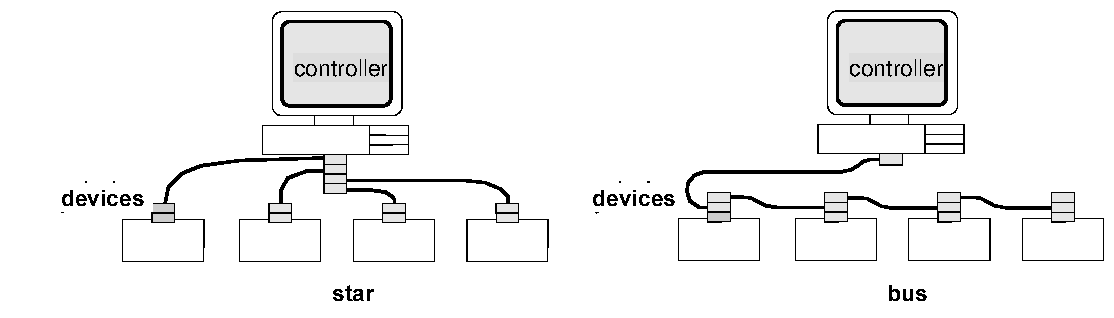
\includegraphics[width=10cm]{./wyklady/IEEE488_SCPI_2_1.pdf}\\
\textbf{Podział urządzenia systemowego na cześć interfejsową i urządzenie właściwe}\\
Można tak podzielić każde urządzenie wykonawcze. Część interfejsowa to zdolność urządzenia do wymiany komunikatów z innymi elementami systemu, a urządzenie właściwe wykonuje podstawowe funkcje urządzenia.\\
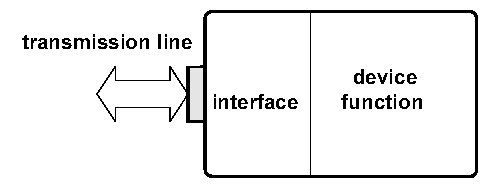
\includegraphics[width=8cm]{./wyklady/IEEE488_SCPI_2_2.pdf}

\newpage
\subsubsection{Magistrala}
\begin{wrapfigure}{r}{0.5\textwidth}
	\vspace{0pt}
	\begin{center}
		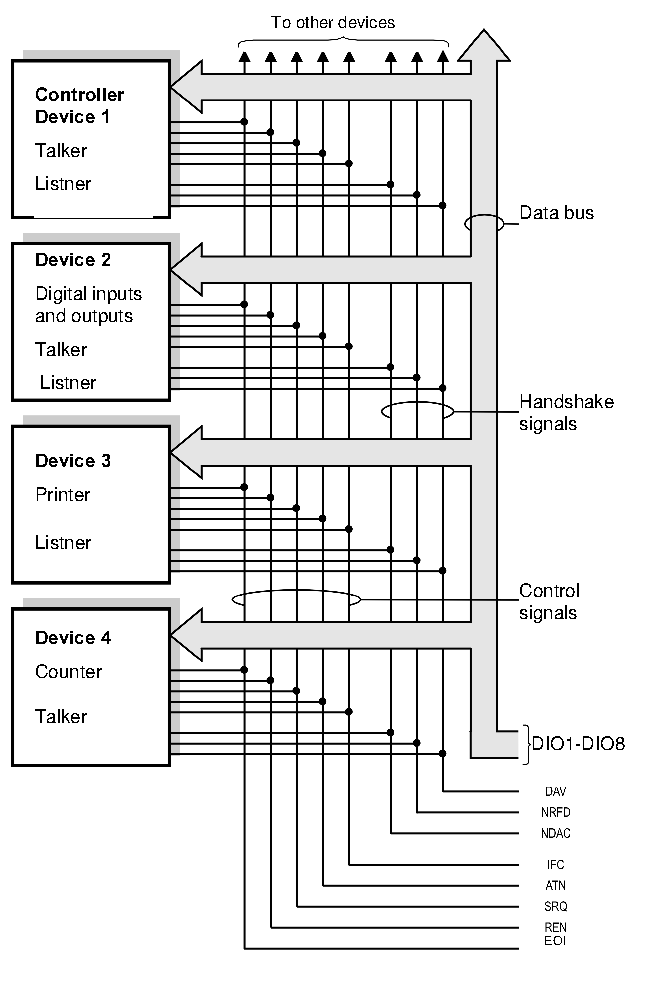
\includegraphics[width=0.40\textwidth]{./wyklady/IEEE488_SCPI_3_1.pdf}
	\end{center}
	\vspace{-20pt}
	\caption{Reprezentacja magistrali}
	\vspace{-10pt}
\end{wrapfigure}

\textbf{Właściwości}
\begin{itemize}
	\item Magistrala zawiera 16 linii
	\begin{itemize}
		\item 8 dla transmisji danych
		\item 8 dla sygnałów sterujących
	\end{itemize}
	\item Jest to łącze równoległe, umożliwia przesłanie wszystkich bitów bajtu
	\item DIO1-DIO8 – dwukierunkowa magistrala danych
	\item 5 sygnałów kontrolnych:
	\begin{itemize}
		\item ATN (\emph{Attention} - wyjście), określa tryb pracy magistrali danych
		\begin{itemize}
			\item ATN=0 - transmisja bajtów danych
			\item ATN=1 - transmisja instrukcji sterujących (adresów lub rozkazów)
		\end{itemize}
		\item REN (\emph{Remote Enable} – wyjście), 1 oznacza, że system jest zarządzany zdalnie przez kontroler
		\item IFC (\emph{Interface clear} – wyjście), 1 powoduje wyzerowanie części interfejsowych urządzeń
		\item SRQ (\emph{Service request} – wejście), 1 oznacza, że w systemie jest co najmniej jedno urządzenie żądające obsługi
		\item EOI (\emph{End Or Identity} – wyjście or wejście), zależny od stanu linii ATN
		\begin{itemize}
			\item EOI=1 razem z ATN=0 (EOI=1 $\XOR$ ATN=0) - realizacja znacznika końca bloku danych
			\item EOI=1 razem z ATN=1 (EOI=1 $\XOR$ ATN=1) – kontrola równoległa
		\end{itemize}
	\end{itemize}
	\item 3 sygnały sterujące (\emph{Byte handshake signals})
	\begin{itemize}
		\item NRFD (\emph{Not Ready For Data} – wyjście or wejście) - jest co najmniej jeden odbiorce niegotowy do przyjęcia danych
		\item DAV (\emph{Data Valid} – wyjście or wejście) - bajt znajdujący się na magistrali jest ważny i może zostać odczytany
		\item NDAC (\emph{Not Data Accepted} – wyjście or wejście) - przyjęcia bajtu na magistrali nie zostało potwierdzone przez wszystkich odbiorców
	\end{itemize}
\end{itemize}
\newpage
\subsubsection{Funkcje interfejsowe}
Każda funkcja reprezentuje pewną określoną zdolność urządzenia jako jednostki systemu GPIB.\\
Ciekawostka: każda funkcja implementowana jest tylko w tych urządzeniach, które jej potrzebują.
\begin{itemize}
	\item SH (\emph{Source Handshake}) - inicjator transmisji, dla urządzeń mogących nadawać dane
	\item AH (\emph{Acceptor Handshake}) - akceptor transmisji, dla urządzeń mogących odbierać dane
	\item T (\emph{Talker}) - nadawca, umożliwienie wprowadzenia bajtu na magistralę danych
	\item L (\emph{Listener}) - odbiorca, umożliwienie odebranie bajtu z magistrali danych
	\item SR (\emph{Service Request}) - zgłoszenie żądania obsługi
	\item DC (\emph{Device Clear}) - zerowanie urządzenia, umożliwienie zdalnego zerowania (reset)
	\item DT (\emph{Device Trigger}) - wyzwalanie urządzenia, umożliwienie zdalnego wyzwolenia operacji (pomiaru)
	\item RL (\emph{Remote/Local}) - zdalne / lokalne, umożliwienie przełączania trybu urządzenia
	\item PP (\emph{Parallel Poll}) - kontrola równoległa, wszystkie linie danych mogą odbierać żądania. Każde urządzenie ma przypisaną linię danych. 
	\item C (\emph{Controller}) - kontroler, umożliwienie zdalnego zarządzania systemem GBIB i przekazywanie zarządzania innym kontrolerom - w systemie może być wiele kontrolerów, jednak tylko jeden może być aktywny, reszta musi być uśpiona.
\end{itemize}

\subsubsection{Podział komunikatów}
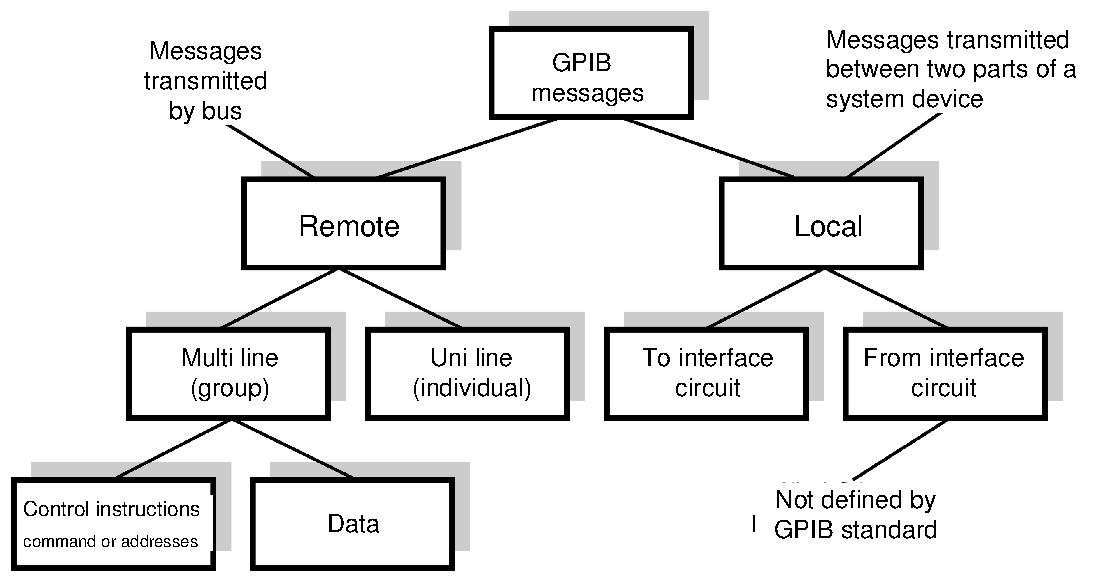
\includegraphics[width=10cm]{./wyklady/IEEE488_SCPI_8_1.pdf}\\\\
komunikaty dzielimy na zdalne(przesyłane po magistrali)  i lokalne (wymieniane między częścią interfejsowa, a urządzeniem właściwym).\\
Komunikaty zdalne dzielimy na:
\begin{itemize}
	\item wieloliniowe: przenoszone przez magistrale danych. Tutaj wyróżniamy:
	\begin{itemize}
		\item instrukcje sterujące (adresy lub rozkazy)
		\item dane
	\end{itemize}
	\item jednoliniowe: przenoszone przez wydzieloną linię sterującą
\end{itemize}
\newpage
\textbf{Podział funkcjonalny komunikatów}:
\begin{itemize}
	\item UC (\emph{Universal Commands}) - rozkazy uniwersalne, przeznaczone dla wszystkich urządzeń w systemie
	\item AC (\emph{Addressed Commands}) - rozkazy adresowane, przeznaczona tylko na konkretnych urządzeń
	\item AD (\emph{Addresses}) - adresy, komunikaty umożliwiające wyznaczenie urządzenia nadającego i urządzeń odbierających
	\item HS (\emph{Handshake}) - komunikaty synchronizacji, kontrolujące transfer bajtu przez magistralę danych
	\item DD (\emph{Device Depended} (data)) - komunikaty zależne od urządzenia, ich znaczenie jest zależne od przyrządu
	\item ST (\emph{Status}) - komunikaty statusowe, udostępniają informacje o stanie urządzenia
	\item SE (\emph{Secondary}) - komunikaty wtórne, adres lub rozkaz wtórny
\end{itemize}

\subsubsection{Złącze interfejsu (connector)}
\begin{wrapfigure}{r}{0.5\textwidth}
	\vspace{0pt}
	\begin{center}
		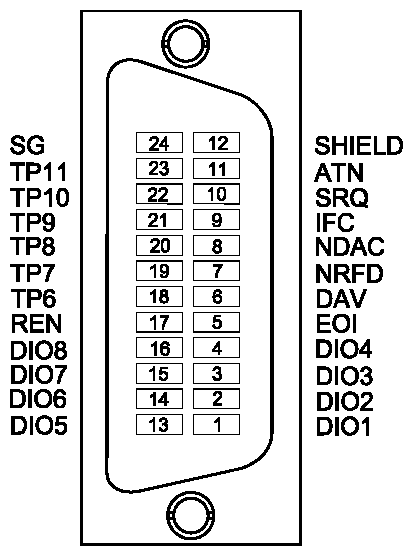
\includegraphics[width=0.30\textwidth]{./wyklady/IEEE488_SCPI_11_1.pdf}
	\end{center}
	\vspace{-20pt}
	\caption{Złącze}
	\vspace{-10pt}
\end{wrapfigure}
W systemie GPIB zastosowano 24-stykowe złącze.
\begin{itemize}
	\item Wszystkie sygnały mają wspólny potencjał odniesienia (masę SG).
	\item Linie sterujące: DAV, NRFD, NDAC, IFC, SRQ oraz ATN są wykonane w postaci skręcanej pary przewodów, w któryc przewód powrotny jest podłączony odpowiednio do punktów TP1, TP2, ... TP11.
	\item Zacisk SHIELD stanowi kontakt do podłączenia ekranu kabla.
\end{itemize}

\subsubsection{Schemat blokowy interfejsu GPIB}
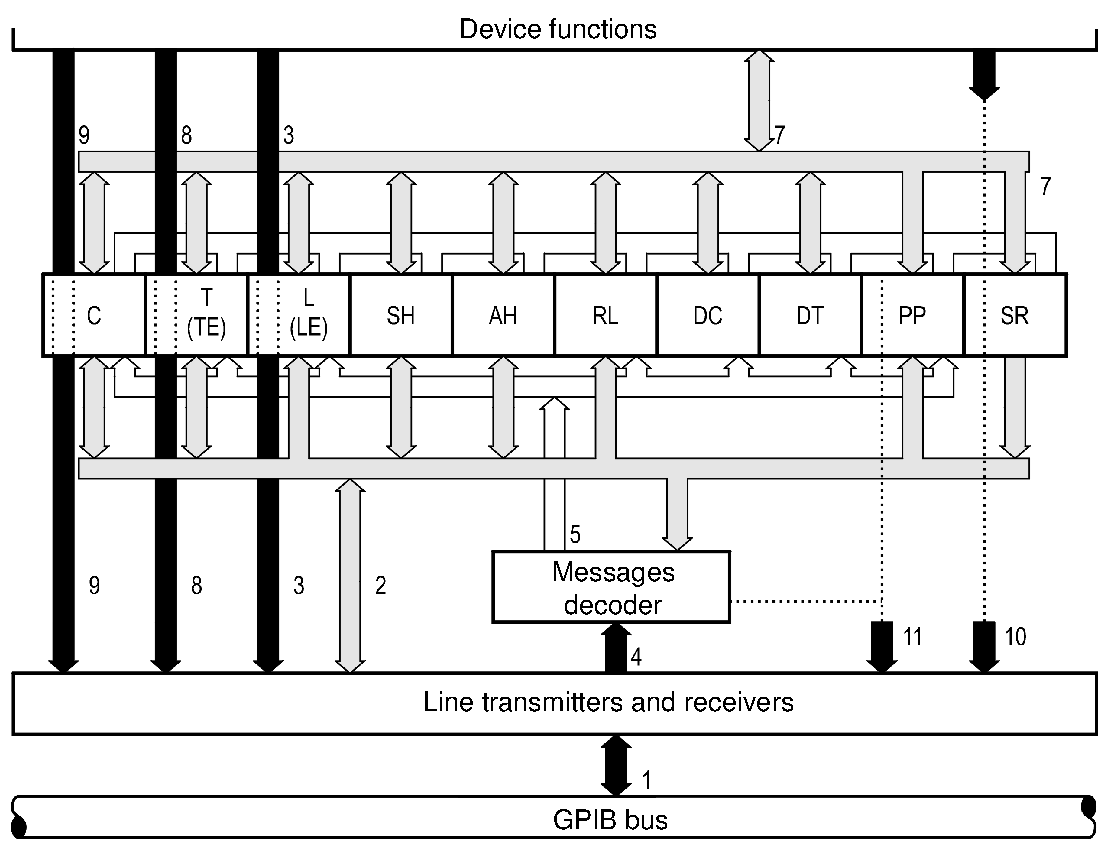
\includegraphics[width=10cm]{./wyklady/IEEE488_SCPI_12_1.pdf}

% ==============================================================
% --- Standard IEEE-488.2
% ==============================================================
\subsection{Standard IEEE-488.2}
Standard ten określa:
\begin{itemize}
	\item Protokół wymiany komunikatów pomiędzy kontrolerem, a urządzeniem na poziomie warstwy 2
	\item Synchronizację działania kontrolera i urządzenia
	\item Strukturę systemu statusowego w urządzeniu i sposób jego obsługi
	\item Zestaw tzw. rozkazów wspólnych
\end{itemize}

\subsubsection{Schemat funkcjonalny urządzenia}
Ilustracja przepływu danych i ich przetwarzania\\
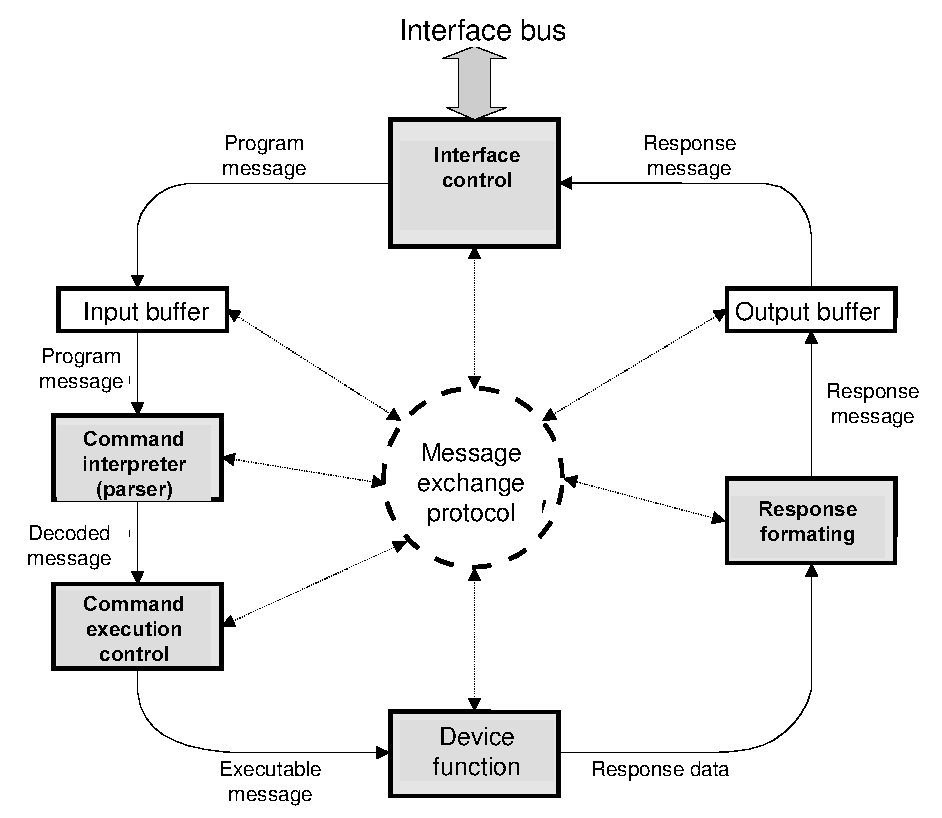
\includegraphics[width=9cm]{./wyklady/IEEE488_SCPI_19_1.pdf}

\subsubsection{Protokół wymiany komunikatów}
Jego zadaniem jest zapewnienie poprawnego transferu wiadomości pomiędzy kontrolerem, a urządzaniem i określenie reakcji urządzenia na naruszenia reguł protokołu.\\
Ogółem komunikacja pomiędzy kontrolerem a urządzeniem polega na:
\begin{itemize}
	\item wysyłaniu do urządzenia komunikatów programujących, które można podzielić na rozkazy bez odpowiedzi i zapytania
	\item odbieraniu odpowiedzi z urządzenia na wysłane zapytania
\end{itemize}
\textbf{Zasady komunikacji kontrolera z urządzeniem (\emph{Device responsibility})}
\begin{enumerate}
	\item Rozkazy są wykonywane przez urządzenie zgodnie z kolejnością ich wprowadzenia do przyrządu (poza ściśle określonymi wyjątkami)
	\item Urządzenie jest zobowiązane odesłać odpowiedź tylko na wcześniej odebrane zapytanie (przez kontroler)
	\item Odpowiedzi na zapytania są odsyłane w kolejności odpowiadającej odebranym zapytaniom
\end{enumerate}
\newpage
\textbf{Reguły protokołu komunikacyjnego (\emph{Controller responsibility})}
\begin{enumerate}
	\item Kontroler nie może odebrać odpowiedzi na zadane zapytanie, zanim nie zakończy rozpoczętego komunikatu programowego.
	\item Kontroler nie może wysłać kolejnego komunikatu programowego, jeżeli nie odebrał w całości wszystkich odpowiedzi na zadane wcześniej zapytania.
	\item Kontroler nie może podejmować próby odczytu odpowiedzi z urządzenia, jeżeli wcześniej nie wysłał żadnego zapytania.
	\item Zapytanie powodujące odesłanie odpowiedzi o nieokreślonym rozmiarze musi być umieszczone jako ostatnie zapytanie w komunikacie programowym (zawierającym kilka zapytań).
	\item Istnieje niebezpieczeństwo zablokowania urządzenia w przypadku wprowadzenia do urządzenia komunikatu programowego zawierającego kilka zapytań.
\end{enumerate}

% ==============================================================
% --- Standard SCPI
% ==============================================================
\subsection{Standard SCPI}
SCPI (\emph{Standard Commands for Programmable Instruments}), normalizuje treści komunikatów przepływających pomiędzy kontrolerem, a urządzeniem. Można go uważać za język kontroli, określono w nim budowę i reguły syntaktyczne komunikatów programowych wysyłanych do urządzenia i odpowiedzi z urządzenia.\\
Wywodzi się z normy IEEE-488.2.

\subsubsection{Budowa komunikatów}
komunikaty składają się z jednego lub kilku komunikatów jednostkowych. Na końcu komunikatu programowego musi wystąpić znacznik terminujący.\\
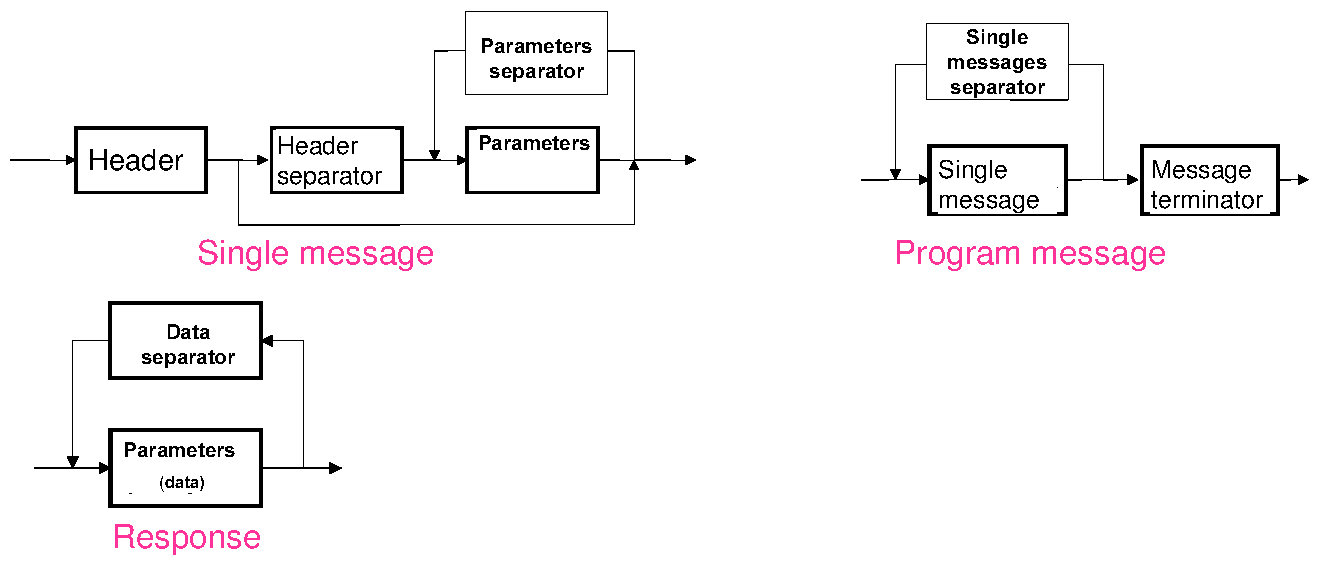
\includegraphics[width=10cm]{./wyklady/IEEE488_SCPI_21_2.pdf}\\\\
\textbf{Komunikat programowy}:
\begin{itemize}
	\item \textbf{Nagłówek}: tekst okreslający znaczenie komunikatu. Może to być pojedyncze słowo kluczowe lub ciąg słów oddzielonych znakiem dwukropka (':', 3Ah)
	\item \textbf{Separator nagłówka}: występuje pomiędzy nagłówkiem, a pierwszym parametrem jako jeden lub kilka znaków niedrukowalnych ASCII z zakresu od 0 do 31 (dec), oprócz NL, 0Ah. Najczęściej jest to jedna lub kilka spacji.
	\item \textbf{Parametry}: określają wartości związane z rozkazem. Separatorem pomiędzy parametrami jest znak przecinka (',', 2Bh), przy czym białe znaki sa ignorowane.
	\item \textbf{Separator komunikatów jednostkowych}: jest to znak średnika (';', 3Bh)
	\item \textbf{Terminator komunikatu}: znacznik terminujący, który jest wymagany do zakończenia komunikatu. Jest to znak LF (NL, 0Ah)
\end{itemize}
\textbf{Odpowiedź}:
\begin{itemize}
	\item Zawierają tylko dane,  
	\item a reszta jak w powyższym
\end{itemize}
\textbf{Zapytanie}:
\begin{itemize}
	\item Nagłówki zapytań mają na końcu znak pytajnika ('?', 3Fh)
\end{itemize}
\textbf{Komunikaty wspólne}:
\begin{itemize}
	\item Posiadają prefiks w postaci znaku gwiazdki ('*', 2Ah)
\end{itemize}
\textbf{Drzewiasta struktura rozkazów SCPI} (jest to to fragment drzewa podsystemu [SENSe]):\\
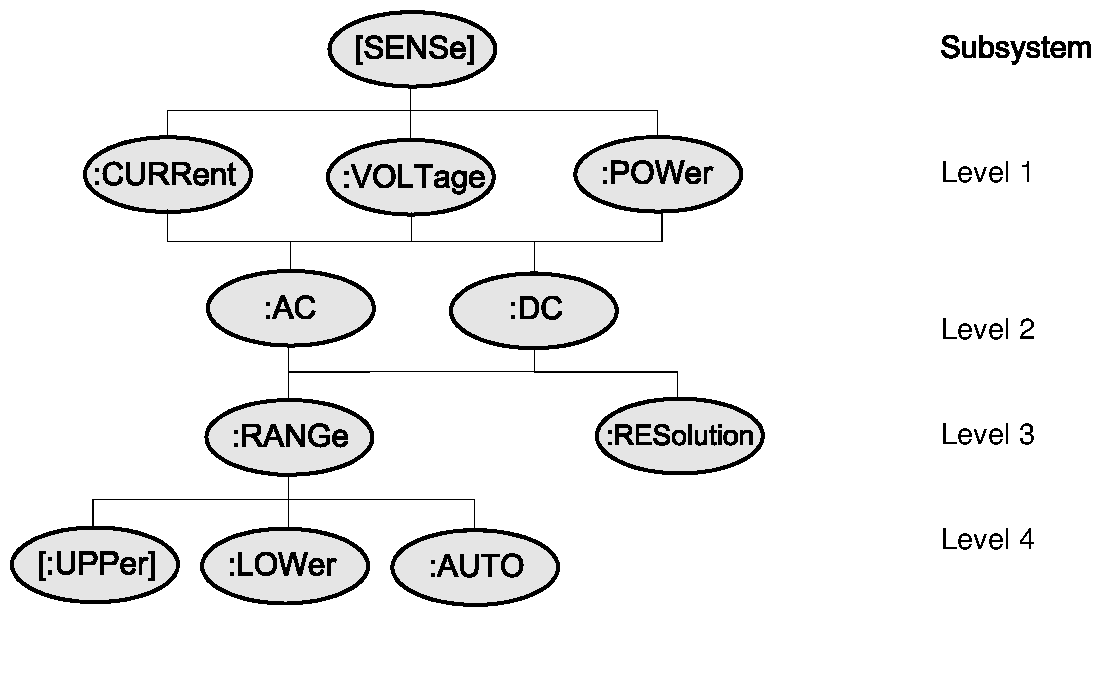
\includegraphics[width=9cm]{./wyklady/IEEE488_SCPI_22_1.pdf}

\subsubsection{Model urządzenia w standardzie SCPI}
Schemat blokowy ilustrujący przepływ sygnału i danych w urządzeniu. Poszczególne bloki reprezentują podstawowe funkcje urządzenia, a ich nazwy są jednocześnie nazwami grup rozkazów (podsystemów), które obsługują daną funkcjonalność.\\
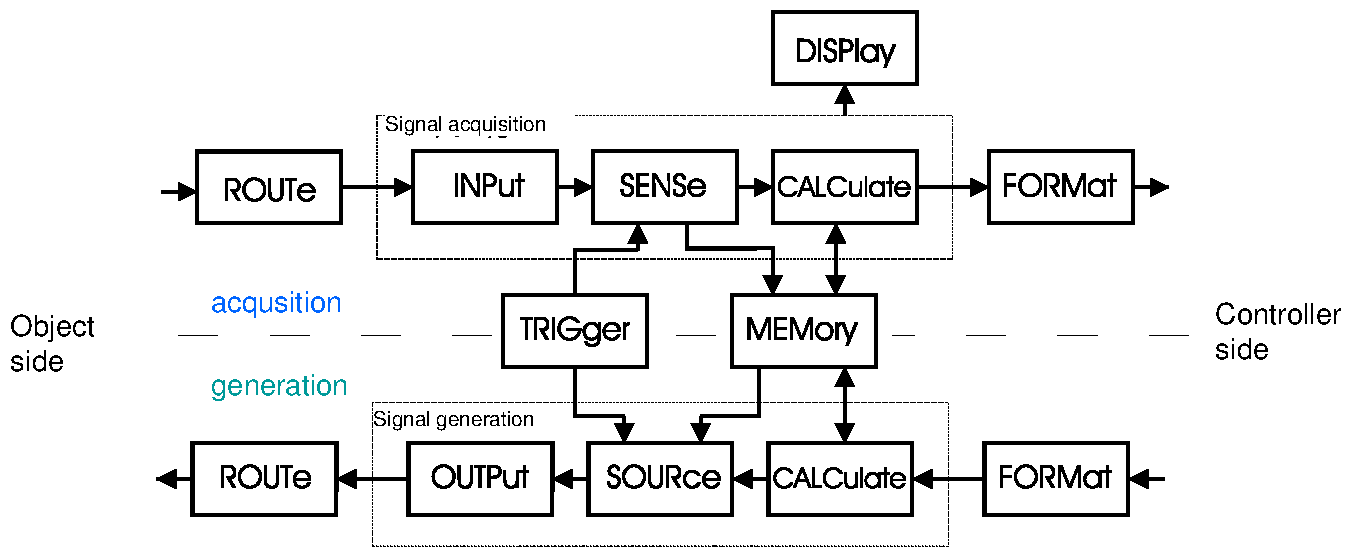
\includegraphics[width=9cm]{./wyklady/IEEE488_SCPI_23_1.pdf}\\
Wyróżnia się dwie części:
\begin{itemize}
	\item akwizycję sygnału ("czujnik")
	\item generację sygnału ("źródło")
\end{itemize}

\subsubsection{Podsystemy w standardzie SCPI}
Podsystem to grupa funkcjonalności. W każdym konkretnym urządzeniu występują tylko te, które są mu potrzebne.\\
Owych podsystemów jest kilkanaście, tutaj są przedstawione najistotniejsze:
\begin{itemize}
	\item \textbf{CALCulate} - odpowiedzialny za matematyczne przetwarzanie wyników i danych po akwizycji sygnału lub przed generacją sygnału
	\item \textbf{INput} - przekształcanie sygnału (wzmocnieniem, filtracją itp.) przed właściwą konwersją dokonywaną w bloku SENSe
	\item \textbf{OUTput} - kontrola przekształtników sygnału wyjściowego (po generacji przez blok SOURce)
	\item \textbf{ROUTe} - odpowiedzialny za podłączenie sygnału wejściowego do układu przekształcającego sygnał lub wyjściowego do zacisków wyjściowych przyrządu
	\item \textbf{SENSe} - kontrola podstawowego modułu akwizycji sygnału (bloku wykonującego konwersję analogowo-cyfrową)
	\item \textbf{SOURce} - kontrola modułu generacji sygnału
	\item \textbf{SYSTem} - podsystem umożliwiający "utrzymanie" przyrządu (kontrolę pomocniczych parametrów)
\end{itemize}

Wyżej wymienione słowa kluczowe mogą występować zarówno w postaci rozwiniętej (np. \textbf{Calculate}), jak i skróconej (\textbf{CALC}).

\subsubsection{Parametry}
Typy parametrów w komunikatach programowych i odpowiedziach zostały określone w standardzie IEEE-488.2, natomiast w SCPI wyróżniono kilka klas parametrów w ramach wybranych typów IEEE-488.2.\\
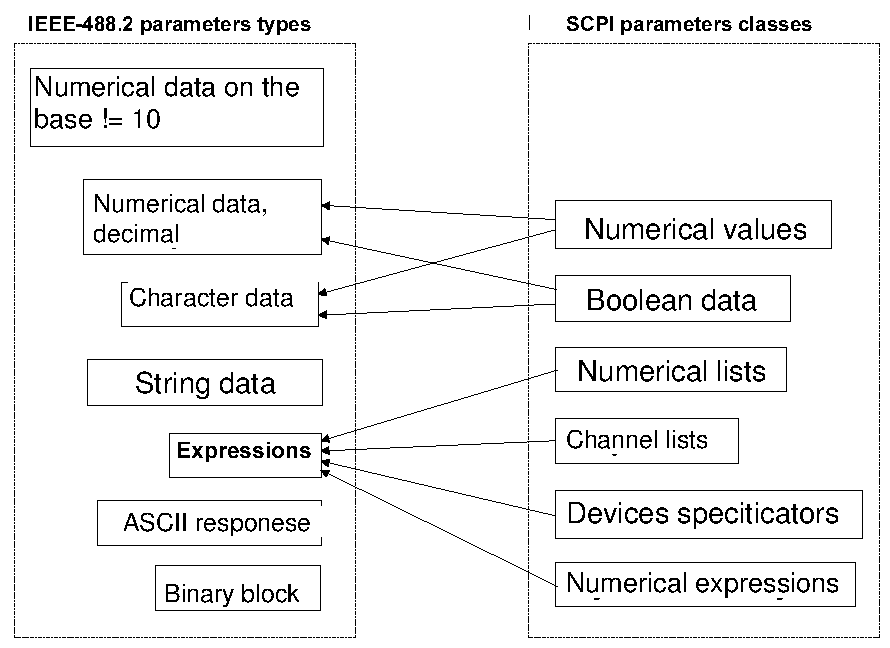
\includegraphics[width=9cm]{./wyklady/IEEE488_SCPI_30_1.pdf}

\subsubsection{Kontrola urządzeń}
Urządzenie kontrolowane przez rozkazy SCPI\\
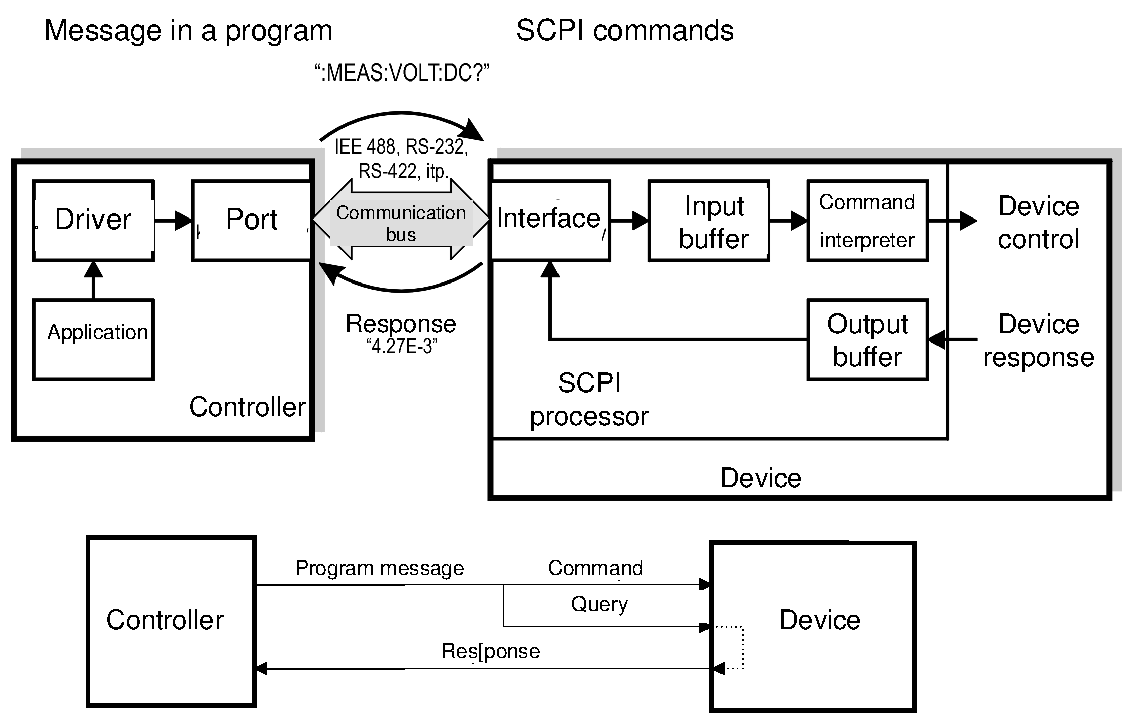
\includegraphics[width=10cm]{./wyklady/IEEE488_SCPI_16_1.pdf}

\newpage
\subsubsection{System rejestrów statusu}
Urządzenie przechowuje informację o stanie w tzw. SRS, który ma strukturę hierarchiczną, złożoną z 5 grup rejestrowych. Każda z nich składa się z rejestru zdarzeń i rejestru maski.
\begin{enumerate}
	\item Bajt statusowy - umieszczona w najwyższym poziomie hierarchii, udostępnia uogólnioną informacje o stanie urządzenia.
	\item Rejestr zdarzeń standardowych - 8-bitowy rejestr na drugim poziomie hierarchii, informuje o wystąpieniu zdarzeń uważanych za "typowe" dla urządzenia SCPI.
	\item Rejestr znaczników urządzenia - 16-bitowy rejestr na drugim poziomie hierarchii, informuje o "jakości" wyników pomiaru i sprawności ważniejszych układów w przyrządzie.
	\item Rejestr operacji - 16-bitowy rejestr na drugim poziomie hierarchii informujący o stanie wykonywanych przez przyrząd operacji.
	\item Rejestr statusu zależny od urządzenia - specyficzny dla urządzenia, liczba i znaczenie bitów są od niego zależne.
\end{enumerate}
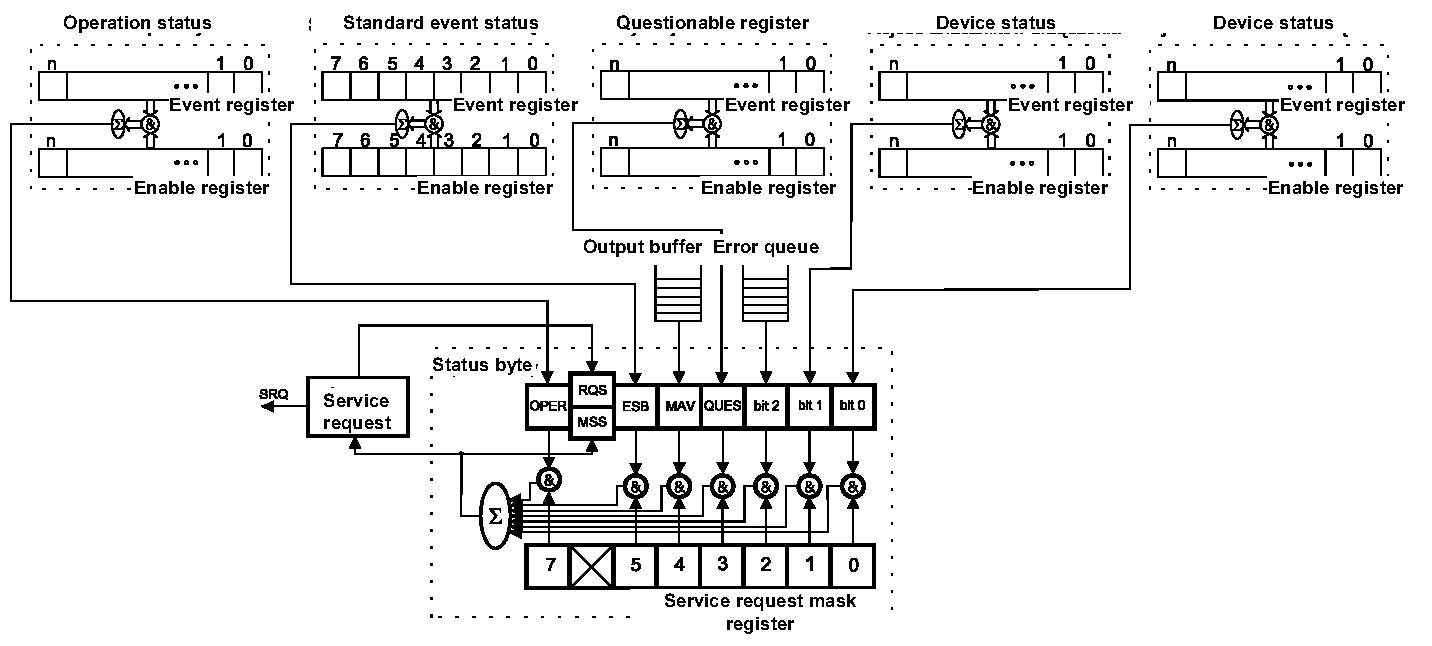
\includegraphics[width=9cm]{./wyklady/IEEE488_SCPI_32_1.pdf}\\\\
Minimal SCPI status system\\
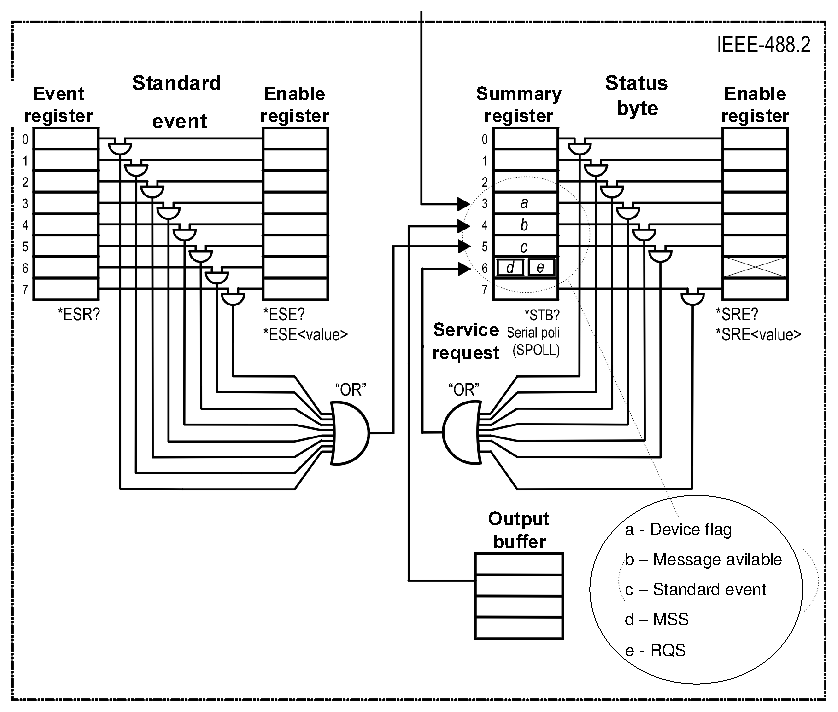
\includegraphics[width=9cm]{./wyklady/IEEE488_SCPI_33_1.pdf}
\newpage
\subsubsection{Synchronizacja urządzeń z aplikacją w standardzie SCPI}
Zadaniem synchronizacji jest zapewnienie właściwej sekwencji operacji urządzeń w systemie.\\
W urządzeniach SCPI synchronizacja aplikacji sterującej z operacjami wykonywanymi przez urządzenie oparta jest na rozkazach *OPC, *OPC? oraz *WAI.\\
\textbf{Rodzaje rozkazów}
Dzielimy je na:
\begin{itemize}
	\item Sekwencyjne - wykonywane jeden po drugim w kolejności wprowadzania ich do przyrządu.
	\item Nakładające się - możliwe wykonywanie wielu rozkazów jednocześnie.
\end{itemize}
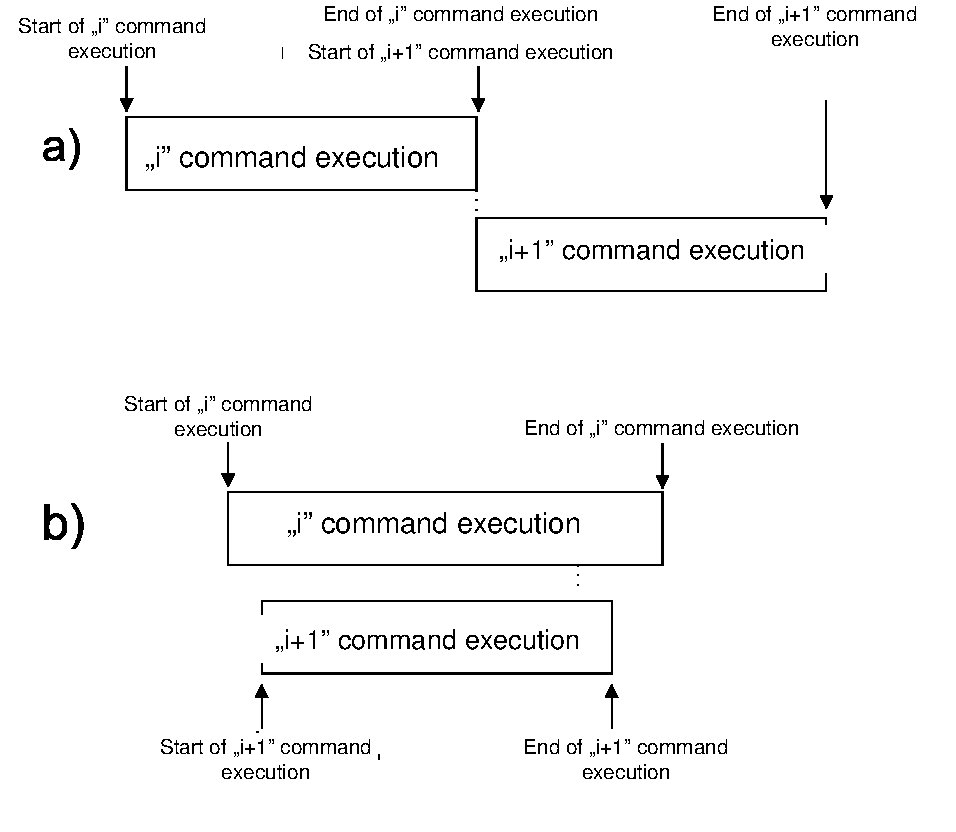
\includegraphics[width=11cm]{./wyklady/IEEE488_SCPI_37_1.pdf}\\\\
\textbf{Rozkazy *OPC, *OPC? oraz *WAI}\\
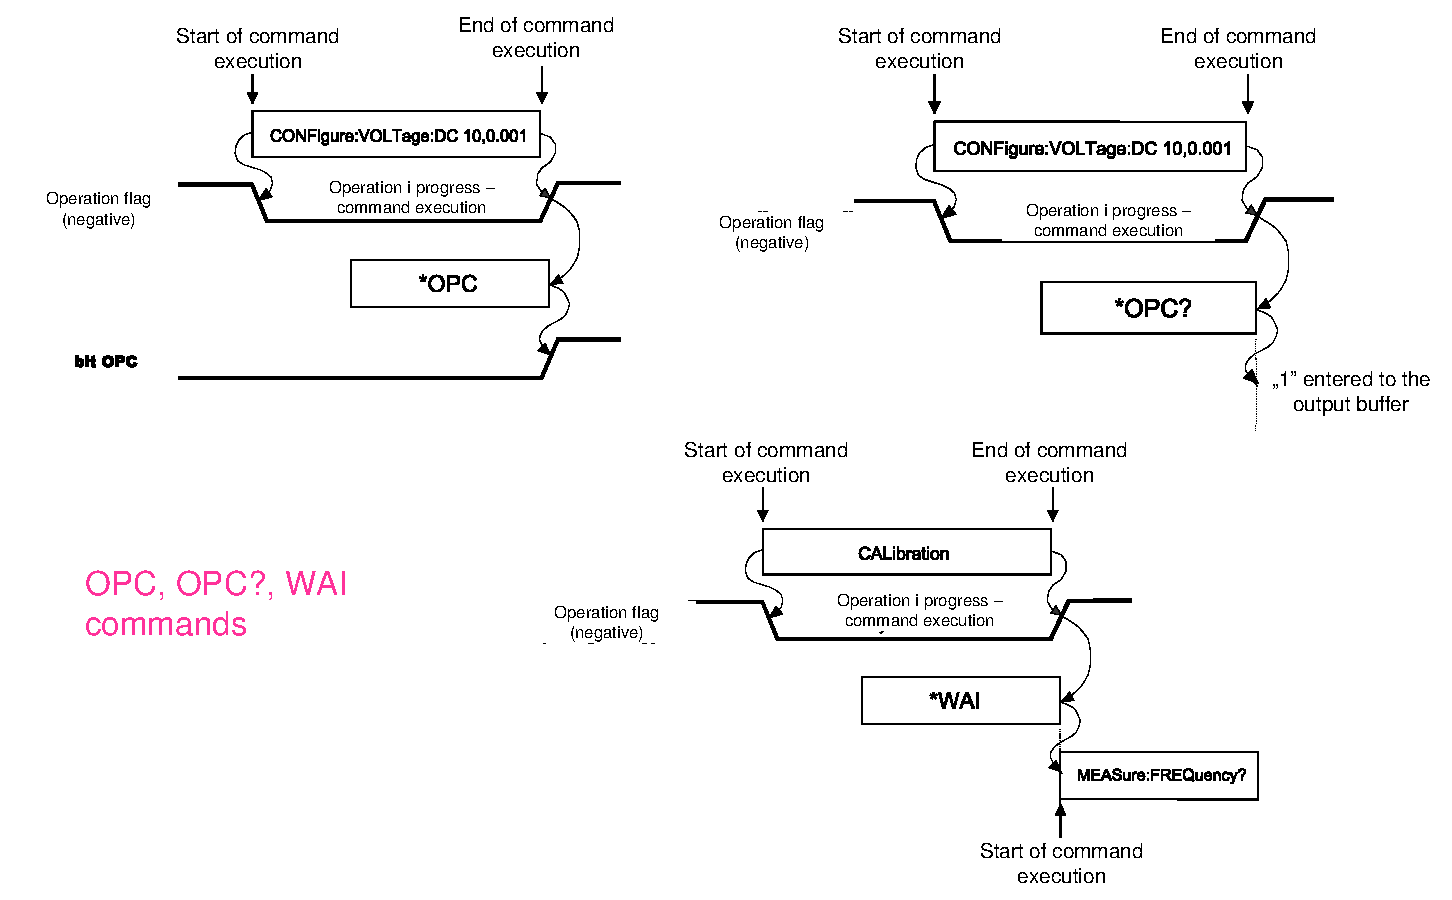
\includegraphics[width=11cm]{./wyklady/IEEE488_SCPI_38_1.pdf}
\newpage
\subsubsection{Wyzwalanie operacji (device trigger)}
Standard SCPI umożliwia uzależnienie wyzwolenia od spełnienie szeregu warunków i wystąpienia róznych zdarzeń (elastyczność).\\
Typowy układ wyzwalania operacji (trigger circuit in HP-34401A multimeter)\\
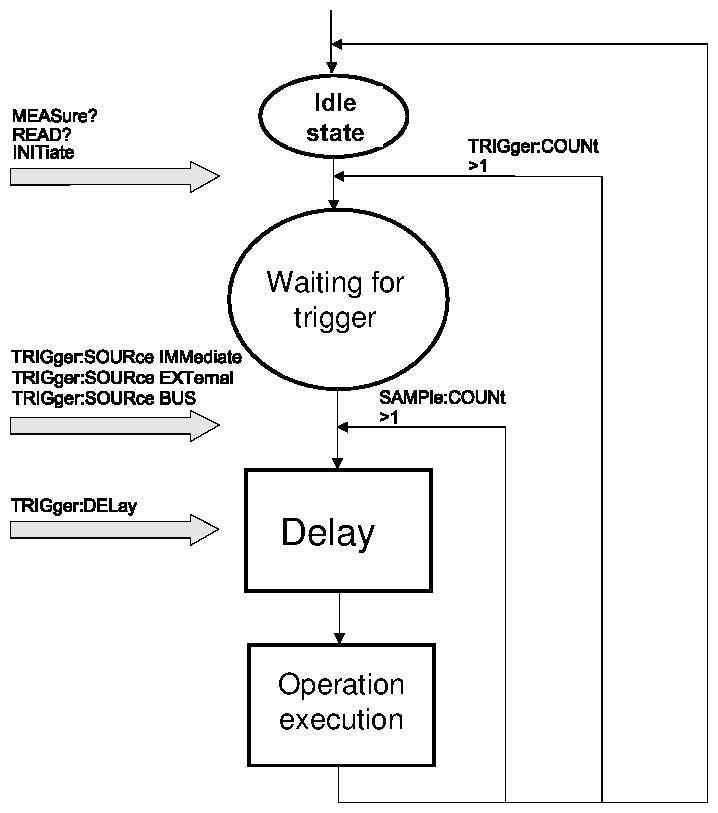
\includegraphics[width=10cm]{./wyklady/IEEE488_SCPI_39_1.pdf}
